\section{Motivations}
\label{sec:motivation}

We focus on computation-heavy ML applications that is beyond the capability of
local devices. Offer some concrete numbers here. Mention that many approaches in
application domains are improving accuracy at a cost of increased
computation. And the spectrum of accuracy-cost is common in these applications.

Also describe application benchmark data set here.

For Face, we use FDDB dataset.

Motivated by the above applications, we outline the key challenges of exploiting
accuracy-cost trade-off for prediction serving and describe how \sysname{}
addresses these challenges.

\subsection{Heterogeneous Environment}

\begin{table}
  \centering
  \begin{tabular}{c c c}
    \toprule
    \specialcell{RPi\\Model B}
    & \specialcell{Macbook \\ Model A1502}
    & \specialcell{Workstation\\Xeon E5-1620} \\
    \midrule
    4105 & 544 & 346 \\
    \bottomrule
  \end{tabular}
  \caption{Processing times (ms) on different platforms.}
\end{table}

Our target application environment consists of machines with large range of
computing resources. $(i)$ End-devices, like mobile phones or IoT platforms, are
significantly limited in their computing power. Performing ML inference often
take seconds to complete. $(ii)$ Edge and Cloud. Both the edge and the cloud
suffers from variable latency, unstable connection, and service contention to
provide consistent response times, especially for 99\% requests.

There is a dizzying array of platforms ranging from \$5 Raspberry Pi to \$1000+
GPU-powered workstation~\cite{zhang2015cloud}.  Even in the cloud, there are
various VM options in the cloud: companies rent VMs based on budget or because
of a lack of expertise.

\textbf{Solution:} Because of the such heterogeneity, we hypothesis an ensemble
of available resources (\autoref{fig:dr}) can overcome the shortcomings of
individual platforms and offer end-users with bounded response times, similar to
prior solutions in both cloud-offloading (Tango~\cite{gordon2015accelerating})
and straggler mitigation in the cloud
(Dolly~\cite{ananthanarayanan2013effective}).

\subsection{Complex Performance Model}
\label{sec:comp-perf-model}

\begin{figure}[t]
  \centering
  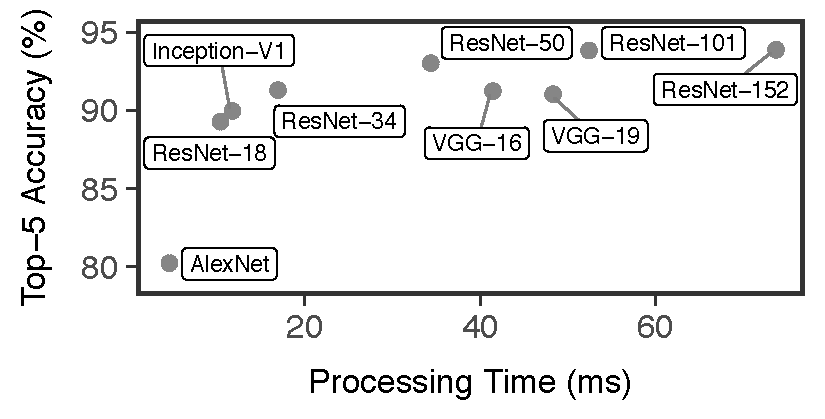
\includegraphics[width=.9\columnwidth]{figures/tradeoff-cnn.pdf}
  \caption{Accuracy-cost trade-off for different CNNs.}
  \label{fig:motiv-functions}
\end{figure}

\begin{figure}[t]
  \centering
  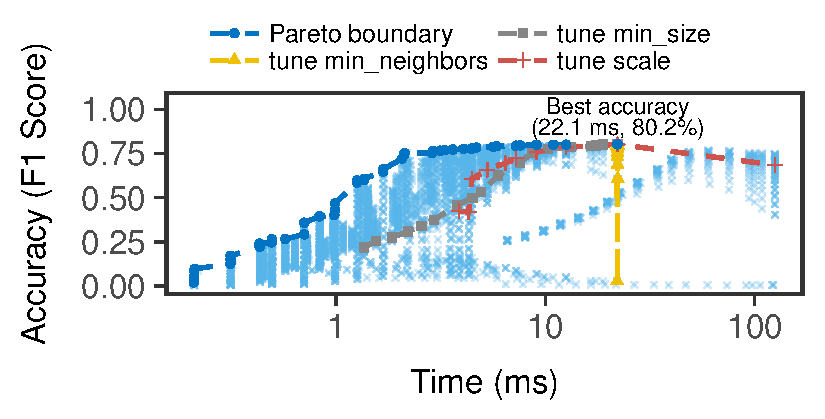
\includegraphics[width=.9\columnwidth]{figures/exhaustive-face.pdf}
  \caption{Complex performance model: spanning multiple dimensions and
    exhibiting non-linear relationship.}
  \label{fig:motiv-params}
\end{figure}

For many ML inference task, there exist more than one algorithm, or tunable
parameters for each algorithm with different accuracy and processing times.  We
can speed up computation by providing a less accurate response. This would allow
some computation tractable on end devices and handling more requests on the
edge/cloud.

For example, accuracy-cost trade-offs for object detection using convolutional
neural network (CNN)~\cite{huang2016speed}. \autoref{fig:tradeoff-cnn} shows one
such benchmark~\cite{cnn.benchmarks}.

Many algorithms have large number of knobs to tune that will affect accuracy and
processing cost. We use Viola-Jones (VJ) cascade face
detector~\cite{viola2001rapid} as an example. \autoref{fig:complex-perf-model}
shows the large parameter space with respect to three parameters:
\texttt{min\_size}, \texttt{min\_neighbors}, and \texttt{scale}.

ML algorithms have many tunable parameters. For many algorithms, processing
times and the accuracy may exhibit \textit{non-linear} behavior with respect to
the parameters.

%%% Local Variables:
%%% mode: latex
%%% TeX-master: "../compute"
%%% End:
